% =====================================================================
%  Capítulo 10. Vectores autorregresivos
% =====================================================================
\part{Modelos multivariados}
\chapter[Vectores autorregresivos]{Vectores autorregresivos: causalidad, impulso-respuesta y pronóstico}\label{cap:var}

\section*{Objetivos de aprendizaje}
Al terminar este capítulo, el lector podrá:
\begin{enumerate}[label=\arabic*.,leftmargin=*]
  \item Escribir un VAR($p$) en forma compañera, verificar su estabilidad con los autovalores y obtener su
        representación de medias móviles.
  \item Demostrar que MCO ecuación por ecuación es eficiente en un VAR y elegir el orden con criterios de
        información.
  \item Contrastar la causalidad de Granger con pruebas clásicas y robustas.
  \item Calcular e interpretar respuestas al impulso ortogonalizadas y la descomposición de la varianza del
        error de pronóstico, y reconocer su dependencia del orden de las variables.
  \item Evaluar fuera de muestra si un VAR pronostica mejor que modelos más simples.
\end{enumerate}

\section*{Motivación}
Hasta ahora hemos modelado una serie a la vez. Pero los precios financieros se mueven juntos y se influyen
mutuamente: cuando el S\&P 500 cae, el VIX sube; cuando sube la tasa de interés, las acciones suelen bajar; las
acciones grandes parecen adelantarse a las pequeñas (Capítulo~\ref{cap:eficiencia}). El \emph{vector
autorregresivo} (VAR), propuesto por Sims (1980) como alternativa a los grandes modelos macroeconómicos, trata
todas las variables como endógenas y deja que los datos digan cómo interactúan. Sus herramientas (la
causalidad de Granger, las respuestas al impulso y la descomposición de la varianza) son hoy el lenguaje común
para estudiar la transmisión de choques entre mercados.

\paragraph{Datos del capítulo.} Rendimientos diarios del S\&P 500 y cambios logarítmicos diarios del VIX
(1999--2018, $T=5\,029$); carteras pequeña (S1V3) y grande (S5V3) de la base de French (1949--2017), y una
muestra mensual de EE.\,UU.\ de la base de Shiller (1960--2023) con la inflación, el cambio en la tasa de los
bonos a 10 años y el rendimiento total del S\&P 500.

% ---------------------------------------------------------------------
\section{El modelo VAR}
% ---------------------------------------------------------------------

\begin{definicion}[VAR($p$)]
Un vector $\mathbf y_t$ de $K$ variables sigue un vector autorregresivo de orden $p$ si
\[
  \mathbf y_t=\mathbf c+A_1\mathbf y_{t-1}+A_2\mathbf y_{t-2}+\dots+A_p\mathbf y_{t-p}+\mathbf u_t,
\]
donde $\mathbf c$ es un vector $K\times1$, cada $A_j$ es una matriz $K\times K$ y $\mathbf u_t$ es un ruido
blanco vectorial: $\E[\mathbf u_t]=\mathbf 0$, $\E[\mathbf u_t\mathbf u_t']=\Sigma$ y
$\E[\mathbf u_t\mathbf u_s']=0$ si $t\ne s$.
\end{definicion}

Cada ecuación es una regresión de una variable sobre $p$ rezagos de todas. Con $K=2$ y $p=1$, por ejemplo:
\begin{align*}
  y_{1t} &= c_1+a_{11}y_{1,t-1}+a_{12}y_{2,t-1}+u_{1t},\\
  y_{2t} &= c_2+a_{21}y_{1,t-1}+a_{22}y_{2,t-1}+u_{2t}.
\end{align*}
El coeficiente $a_{12}$ mide cómo el pasado de $y_2$ ayuda a predecir $y_1$. Las innovaciones $u_{1t}$ y
$u_{2t}$ pueden estar correlacionadas: $\Sigma$ no es diagonal. Esa correlación contemporánea es la que obliga,
más adelante, a decidir un orden entre las variables.

\subsection{Forma compañera y estabilidad}

Un VAR($p$) puede escribirse como un VAR(1) apilando los rezagos. Con
$\boldsymbol\xi_t=(\mathbf y_t',\mathbf y_{t-1}',\dots,\mathbf y_{t-p+1}')'$, de dimensión $Kp$,
\[
  \boldsymbol\xi_t=\boldsymbol\nu+F\,\boldsymbol\xi_{t-1}+\mathbf v_t,\qquad
  F=\begin{bmatrix}
      A_1 & A_2 & \cdots & A_{p-1} & A_p\\
      I_K & 0   & \cdots & 0       & 0\\
      0   & I_K & \cdots & 0       & 0\\
      \vdots &  & \ddots &         & \vdots\\
      0   & 0   & \cdots & I_K     & 0
    \end{bmatrix},
\]
con $\boldsymbol\nu=(\mathbf c',\mathbf 0',\dots)'$ y $\mathbf v_t=(\mathbf u_t',\mathbf 0',\dots)'$. Las filas
inferiores de $F$ solo dicen que $\mathbf y_{t-1}$ es $\mathbf y_{t-1}$. La matriz $F$ es la \emph{matriz
compañera}.

\begin{proposicion}[Estabilidad y representación de medias móviles]\label{prop:varma}
Si todos los autovalores de $F$ tienen módulo menor que uno, el VAR es estacionario y
\[
  \mathbf y_t=\boldsymbol\mu+\sum_{i=0}^{\infty}\Psi_i\,\mathbf u_{t-i},\qquad \Psi_0=I_K,\qquad
  \Psi_i=\sum_{j=1}^{\min(i,p)}A_j\Psi_{i-j}\ \ (i\ge1),
\]
donde $\boldsymbol\mu=(I_K-A_1-\dots-A_p)^{-1}\mathbf c$ es la media del proceso.
\end{proposicion}

\begin{proof}
Trabajamos con la forma compañera, en desviaciones respecto de su media $\bar{\boldsymbol\xi}$:
$\tilde{\boldsymbol\xi}_t=F\tilde{\boldsymbol\xi}_{t-1}+\mathbf v_t$. Sustituimos hacia atrás $k$ veces:
\begin{align*}
  \tilde{\boldsymbol\xi}_t &= F\tilde{\boldsymbol\xi}_{t-1}+\mathbf v_t\\
                           &= F\bigl(F\tilde{\boldsymbol\xi}_{t-2}+\mathbf v_{t-1}\bigr)+\mathbf v_t\\
                           &= F^2\tilde{\boldsymbol\xi}_{t-2}+F\mathbf v_{t-1}+\mathbf v_t\\
                           &\;\;\vdots\\
                           &= F^k\tilde{\boldsymbol\xi}_{t-k}+\sum_{i=0}^{k-1}F^i\mathbf v_{t-i}.
\end{align*}
Si $F=VDV^{-1}$ con $D$ diagonal de autovalores $\lambda_\ell$ (el caso general usa la forma de Jordan con el
mismo resultado), entonces $F^k=VD^kV^{-1}$ y cada elemento de $D^k$ es $\lambda_\ell^k\to0$ porque
$|\lambda_\ell|<1$. Así $F^k\tilde{\boldsymbol\xi}_{t-k}\to0$ y
\begin{align*}
  \tilde{\boldsymbol\xi}_t &= \sum_{i=0}^{\infty}F^i\mathbf v_{t-i}.
\end{align*}
Las primeras $K$ filas dan $\mathbf y_t-\boldsymbol\mu=\sum_i\Psi_i\mathbf u_{t-i}$, con $\Psi_i$ el bloque
superior izquierdo de $F^i$. Para la recursión, sustituimos la representación en el VAR e igualamos los
coeficientes de $\mathbf u_{t-i}$ en ambos lados:
\begin{align*}
  \sum_{i\ge0}\Psi_i\mathbf u_{t-i}
     &= \sum_{j=1}^{p}A_j\sum_{m\ge0}\Psi_m\mathbf u_{t-j-m}+\mathbf u_t,\\
  \text{coeficiente de }\mathbf u_t:\quad \Psi_0 &= I_K,\\
  \text{coeficiente de }\mathbf u_{t-i}:\quad \Psi_i &= \sum_{j=1}^{\min(i,p)}A_j\Psi_{i-j}. && \qedhere
\end{align*}
\end{proof}

La forma de las respuestas depende de los autovalores. Si son reales y menores que uno, los efectos de un
choque decaen de forma monótona; si son complejos, $\lambda=re^{\pm i\theta}$, decaen oscilando, con período
$2\pi/\theta$ y amortiguamiento $r^i$; si alguno tiene módulo mayor que uno, explotan. La
Figura~\ref{fig:varautoval} muestra los tres casos con un VAR(1) bivariado. En el panel izquierdo los
autovalores reales $0{,}5$ de los dos primeros casos coinciden en el mismo punto.

\begin{figure}[ht]
\centering
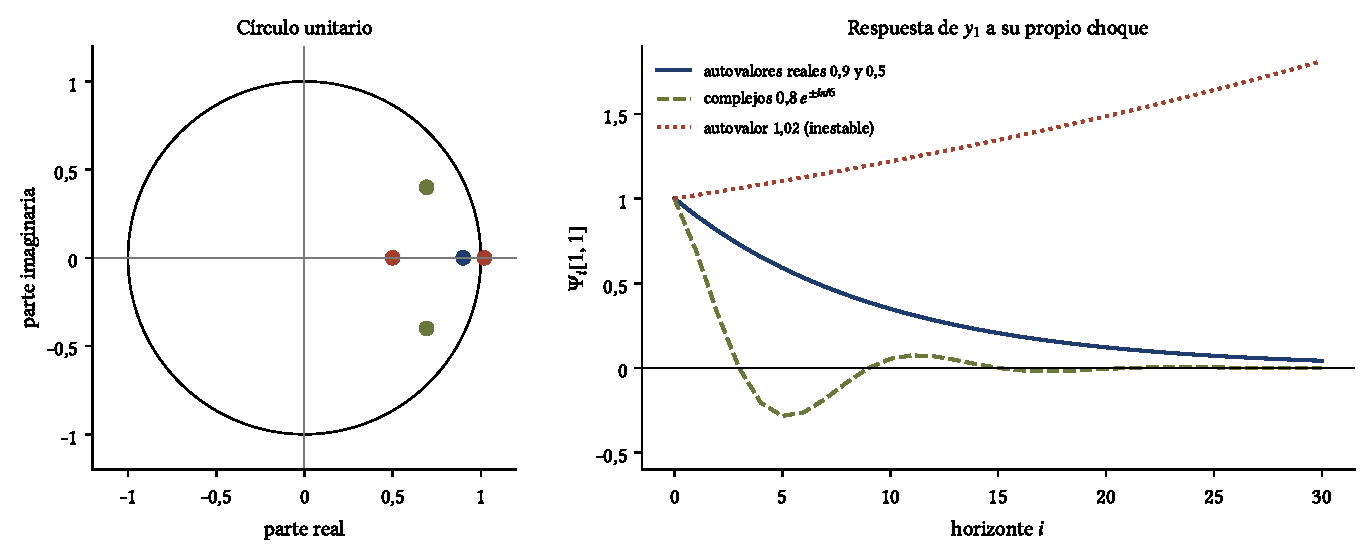
\includegraphics[width=\linewidth]{graficos/cap10_fig_autovalores.pdf}
\caption{Izquierda: autovalores de tres VAR(1) bivariados frente al círculo unitario. Derecha: elemento
$[1,1]$ de $\Psi_i$, la respuesta de $y_1$ a su propia innovación. Autovalores reales dentro del círculo:
decaimiento monótono. Complejos: oscilación amortiguada. Uno fuera del círculo: explosión.}
\label{fig:varautoval}
\end{figure}

% ---------------------------------------------------------------------
\section{Estimación y selección del orden}
% ---------------------------------------------------------------------

Sea $X$ la matriz $n\times(1+Kp)$ cuya fila $t$ es $(1,\mathbf y_{t-1}',\dots,\mathbf y_{t-p}')$ y $Y$ la matriz
$n\times K$ cuya fila $t$ es $\mathbf y_t'$. El VAR se escribe $Y=XB+U$, con
$B=(\mathbf c,A_1,\dots,A_p)'$ de dimensión $(1+Kp)\times K$: cada columna de $B$ contiene los coeficientes de
una ecuación. El estimador de MCO ecuación por ecuación es $\hat B=(X'X)^{-1}X'Y$.

\begin{proposicion}[MCO ecuación por ecuación es MCG]\label{prop:varmco}
Como todas las ecuaciones tienen los mismos regresores, el estimador de mínimos cuadrados generalizados del
sistema, que aprovecha la correlación $\Sigma$ entre ecuaciones, coincide con MCO ecuación por ecuación. Con
errores normales, coincide también con el de máxima verosimilitud.
\end{proposicion}

\begin{proof}
Apilamos las columnas de $Y$ y de $U$ en un solo vector:
$\operatorname{vec}(Y)=(I_K\otimes X)\boldsymbol\beta+\operatorname{vec}(U)$, con
$\boldsymbol\beta=\operatorname{vec}(B)$ y $\Var[\operatorname{vec}(U)]=\Sigma\otimes I_n$. El estimador MCG es
\begin{align*}
  \hat{\boldsymbol\beta}_{\text{MCG}}
    &= \bigl[(I_K\otimes X)'(\Sigma^{-1}\otimes I_n)(I_K\otimes X)\bigr]^{-1}
       (I_K\otimes X)'(\Sigma^{-1}\otimes I_n)\operatorname{vec}(Y).
\end{align*}
Usamos las reglas $(A\otimes B)'=A'\otimes B'$, $(A\otimes B)(C\otimes D)=AC\otimes BD$ y
$(A\otimes B)^{-1}=A^{-1}\otimes B^{-1}$. El término entre corchetes es
\begin{align*}
  (I_K\otimes X')(\Sigma^{-1}\otimes I_n)(I_K\otimes X)
    &= (\Sigma^{-1}\otimes X')(I_K\otimes X)\\
    &= \Sigma^{-1}\otimes X'X,
\end{align*}
y el factor que multiplica a $\operatorname{vec}(Y)$ es
\begin{align*}
  (I_K\otimes X')(\Sigma^{-1}\otimes I_n) &= \Sigma^{-1}\otimes X'.
\end{align*}
Entonces
\begin{align*}
  \hat{\boldsymbol\beta}_{\text{MCG}}
    &= \bigl(\Sigma^{-1}\otimes X'X\bigr)^{-1}\bigl(\Sigma^{-1}\otimes X'\bigr)\operatorname{vec}(Y)\\
    &= \bigl(\Sigma\otimes(X'X)^{-1}\bigr)\bigl(\Sigma^{-1}\otimes X'\bigr)\operatorname{vec}(Y)\\
    &= \bigl(\Sigma\Sigma^{-1}\otimes(X'X)^{-1}X'\bigr)\operatorname{vec}(Y)\\
    &= \bigl(I_K\otimes(X'X)^{-1}X'\bigr)\operatorname{vec}(Y).
\end{align*}
El último operador aplica $(X'X)^{-1}X'$ a cada columna de $Y$, que es MCO ecuación por ecuación. Con errores
normales, maximizar la verosimilitud respecto de $\boldsymbol\beta$ equivale a minimizar la forma cuadrática que
minimiza MCG.
\end{proof}

La matriz de covarianzas de los residuos se estima con $\hat\Sigma=\hat U'\hat U/(n-1-Kp)$, o con $\tilde\Sigma=\hat
U'\hat U/n$ (máxima verosimilitud). El orden $p$ se elige minimizando un criterio de información sobre una
\emph{misma} muestra efectiva para todos los candidatos (se descartan las primeras $p_{\max}$ observaciones):
\begin{align*}
  \text{AIC}(p) &= \ln\bigl|\tilde\Sigma_p\bigr|+\frac{2}{n}\,k,\\
  \text{BIC}(p) &= \ln\bigl|\tilde\Sigma_p\bigr|+\frac{\ln n}{n}\,k,\\
  \text{HQ}(p)  &= \ln\bigl|\tilde\Sigma_p\bigr|+\frac{2\ln\ln n}{n}\,k,
\end{align*}
con $k=pK^2+K$ parámetros. Como en el caso univariado, el BIC penaliza más y elige modelos más parsimoniosos; el
AIC tiende a sobreajustar, pero es preferible si el objetivo es pronosticar.

% ---------------------------------------------------------------------
\section{Causalidad de Granger}
% ---------------------------------------------------------------------

\begin{definicion}[Causalidad de Granger; Granger, 1969]
La variable $y_2$ \emph{no causa en el sentido de Granger} a $y_1$ si el error cuadrático medio del mejor
pronóstico de $y_{1,t+h}$ con la información pasada de $y_1$ y $y_2$ es el mismo que con la de $y_1$ sola, para
todo $h\ge1$.
\end{definicion}

En un VAR bivariado, $y_2$ no causa a $y_1$ si y solo si todos los coeficientes $a_{12}$ de las matrices
$A_1,\dots,A_p$ son cero: entonces la primera ecuación no depende del pasado de $y_2$, y como la ecuación de
$y_1$ no recibe nada de $y_2$, tampoco lo hacen sus pronósticos a cualquier horizonte. La hipótesis se contrasta
en la ecuación de $y_1$ con una prueba $F$:
\[
  F=\frac{(\mathrm{SRC}_r-\mathrm{SRC}_u)/r}{\mathrm{SRC}_u/(n-q)}\sim F_{r,\,n-q},
\]
donde $\mathrm{SRC}_u$ y $\mathrm{SRC}_r$ son las sumas de residuos al cuadrado sin y con la restricción, $r=p$
el número de coeficientes anulados y $q=1+Kp$ el número de regresores. Con rendimientos financieros, que son
heterocedásticos, conviene también la prueba de Wald con la matriz de covarianzas de White (HC0) del
Capítulo~\ref{cap:robustos}:
\[
  W=\hat{\boldsymbol\beta}_R'\bigl[\hat V_{\text{HC0}}\bigr]_R^{-1}\hat{\boldsymbol\beta}_R\ \xrightarrow{d}\ \chi^2_r ,
\]
donde el subíndice $R$ selecciona los coeficientes restringidos.

\begin{observacion}
La causalidad de Granger es \emph{predictiva}, no estructural. Que el pasado de $y_2$ ayude a pronosticar $y_1$
no significa que $y_2$ cause $y_1$ en el sentido económico; puede haber una tercera variable omitida, o bien
$y_2$ puede reaccionar antes a la misma información. En mercados eficientes, además, se espera poca causalidad
de Granger entre precios, porque cualquier predictibilidad tiende a ser explotada.
\end{observacion}

% ---------------------------------------------------------------------
\section{Respuestas al impulso}
% ---------------------------------------------------------------------

La matriz $\Psi_i$ de la Proposición~\ref{prop:varma} da el efecto de una innovación $\mathbf u_t$ sobre
$\mathbf y_{t+i}$. Pero si las innovaciones están correlacionadas, no tiene sentido preguntar qué pasa cuando
``solo'' cambia $u_{2t}$: cuando $u_{2t}$ se mueve, $u_{1t}$ suele moverse también. La solución es expresar
$\mathbf u_t$ en términos de choques no correlacionados.

\begin{proposicion}[Choques ortogonalizados de Cholesky]\label{prop:chol}
Sea $P$ la matriz triangular inferior con diagonal positiva tal que $PP'=\Sigma$ (factor de Cholesky). Los choques
$\boldsymbol\varepsilon_t=P^{-1}\mathbf u_t$ tienen $\Var(\boldsymbol\varepsilon_t)=I_K$, y
\[
  \mathbf y_t=\boldsymbol\mu+\sum_{i=0}^{\infty}\Theta_i\,\boldsymbol\varepsilon_{t-i},\qquad \Theta_i=\Psi_iP .
\]
El elemento $\theta_{kj,i}$ de $\Theta_i$ es la respuesta de $y_k$, $i$ períodos después, a un choque de una
desviación estándar en la variable $j$.
\end{proposicion}

\begin{proof}
La varianza de los choques es
\begin{align*}
  \Var(\boldsymbol\varepsilon_t) &= P^{-1}\,\Var(\mathbf u_t)\,(P^{-1})'\\
                                 &= P^{-1}\,PP'\,(P')^{-1}\\
                                 &= I_K .
\end{align*}
Como $\mathbf u_t=P\boldsymbol\varepsilon_t$, sustituimos en la representación de medias móviles:
\begin{align*}
  \mathbf y_t &= \boldsymbol\mu+\sum_{i=0}^{\infty}\Psi_i\,P\boldsymbol\varepsilon_{t-i}\\
              &= \boldsymbol\mu+\sum_{i=0}^{\infty}\Theta_i\,\boldsymbol\varepsilon_{t-i}. && \qedhere
\end{align*}
\end{proof}

Como $P$ es triangular inferior, $\Theta_0=P$ también lo es: el primer choque afecta a todas las variables en el
mismo período, el segundo a todas menos la primera, y así sucesivamente. Ordenar las variables equivale a
suponer que las primeras no reaccionan en el mismo período a los choques de las últimas. Con $K=2$:
\begin{align*}
  P &= \begin{bmatrix} \sqrt{\sigma_{11}} & 0\\[2pt] \dfrac{\sigma_{12}}{\sqrt{\sigma_{11}}} &
        \sqrt{\sigma_{22}-\dfrac{\sigma_{12}^2}{\sigma_{11}}}\end{bmatrix}.
\end{align*}
Toda la covarianza contemporánea se atribuye al choque de la variable ordenada primero. Si la correlación entre
innovaciones es alta, las respuestas cambian mucho al invertir el orden. La Figura~\ref{fig:varorden} lo
muestra con un VAR(1) con $A_1=\bigl[\begin{smallmatrix}0{,}5&0{,}1\\0{,}3&0{,}6\end{smallmatrix}\bigr]$ y
correlación $0{,}6$ entre innovaciones de varianza 1: con el orden $(y_1,y_2)$, el choque en $y_2$ no mueve a
$y_1$ en el impacto; con el orden inverso, lo mueve en $0{,}6$.

\begin{figure}[ht]
\centering
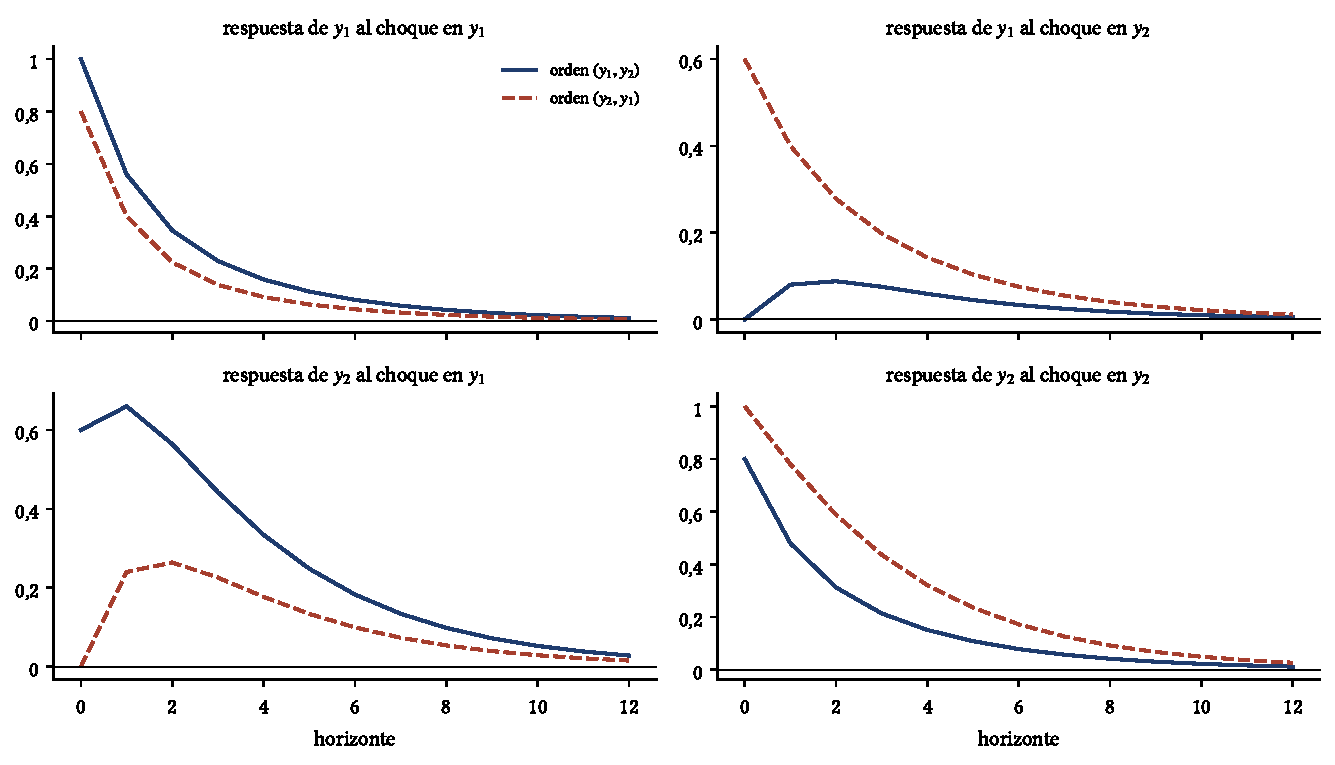
\includegraphics[width=0.92\linewidth]{graficos/cap10_fig_orden.pdf}
\caption{Respuestas ortogonalizadas de un VAR(1) bivariado con innovaciones correlacionadas ($\rho=0{,}6$) según el
orden de Cholesky. La variable ordenada primero recibe toda la correlación contemporánea.}
\label{fig:varorden}
\end{figure}

\paragraph{Alternativas.} Cuando no hay un orden natural, se pueden reportar los dos órdenes, usar las
respuestas \emph{generalizadas} de Pesaran y Shin (1998), que no dependen del orden, o imponer restricciones
basadas en la teoría económica (VAR estructurales). Las bandas de confianza se obtienen por \emph{bootstrap}:
se remuestrean los residuos, se reconstruye la serie con los coeficientes estimados, se reestima el VAR y se
recalculan las respuestas; los percentiles 5 y 95 de las réplicas forman una banda al 90\,\%.

% ---------------------------------------------------------------------
\section{Descomposición de la varianza del error de pronóstico}
% ---------------------------------------------------------------------

\begin{proposicion}[Descomposición de la varianza]\label{prop:fevd}
El error de pronóstico a $h$ períodos de $y_k$ tiene varianza
\[
  \mathrm{ECM}_k(h)=\sum_{i=0}^{h-1}\sum_{j=1}^{K}\theta_{kj,i}^2,
\]
y la proporción debida al choque $j$ es
\[
  \omega_{kj}(h)=\frac{\sum_{i=0}^{h-1}\theta_{kj,i}^2}{\mathrm{ECM}_k(h)},\qquad \sum_{j=1}^{K}\omega_{kj}(h)=1 .
\]
\end{proposicion}

\begin{proof}
El pronóstico óptimo en $T$ es la esperanza condicional. Los choques futuros, de
$\boldsymbol\varepsilon_{T+1}$ a $\boldsymbol\varepsilon_{T+h}$, son impredecibles, y los pasados son conocidos.
El error es entonces la parte de la representación de la Proposición~\ref{prop:chol} que depende de los choques
futuros:
\begin{align*}
  \mathbf y_{T+h}-\E_T[\mathbf y_{T+h}] &= \sum_{i=0}^{h-1}\Theta_i\,\boldsymbol\varepsilon_{T+h-i}.
\end{align*}
Su componente $k$ es
\begin{align*}
  y_{k,T+h}-\E_T[y_{k,T+h}] &= \sum_{i=0}^{h-1}\sum_{j=1}^{K}\theta_{kj,i}\,\varepsilon_{j,T+h-i}.
\end{align*}
Los $\varepsilon_{j,s}$ tienen varianza uno y no están correlacionados entre sí ni en el tiempo, así que la
varianza de la suma es la suma de los cuadrados de los coeficientes:
\begin{align*}
  \mathrm{ECM}_k(h) &= \sum_{i=0}^{h-1}\sum_{j=1}^{K}\theta_{kj,i}^2\,\Var(\varepsilon_{j,T+h-i})\\
                    &= \sum_{j=1}^{K}\Bigl(\sum_{i=0}^{h-1}\theta_{kj,i}^2\Bigr).
\end{align*}
Cada término entre paréntesis es la contribución del choque $j$; dividirla entre el total da $\omega_{kj}(h)$,
y las proporciones suman uno por construcción.
\end{proof}

La descomposición responde a la pregunta: ¿qué fracción de la incertidumbre sobre $y_k$ a $h$ períodos viene de
cada fuente de choques? Hereda del factor de Cholesky la dependencia del orden.

% ---------------------------------------------------------------------
\section{Ejercicios resueltos}
% ---------------------------------------------------------------------

\begin{ejresuelto}{VAR para el S\&P 500 y el VIX}\label{ej:varvix}
\enunciado Con el rendimiento logarítmico diario del S\&P 500, $r_t$, y el cambio logarítmico diario del VIX,
$\Delta v_t$, ambos en porcentaje (1999--2018), elija el orden de un VAR con AIC, BIC y HQ ($p_{\max}=10$),
estime el VAR elegido por el BIC, calcule la correlación de los residuos y verifique la estabilidad.

\solucion
\paso{Paso 1. Selección del orden.} Los tres criterios no coinciden: el AIC elige $p=10$ (el máximo), el HQ
$p=7$ y el BIC $p=2$. Con 5\,029 observaciones, el BIC penaliza cada parámetro con $\ln n/n=0{,}0017$, casi
cuatro veces más que el AIC ($2/n=0{,}0004$). Seguimos al BIC; el Ejercicio~\ref{ej:granger} verifica que las
conclusiones no cambian con $p=7$.

\paso{Paso 2. Estimación.}
\begin{center}\small
\begin{tabular}{@{}lrrrr@{}}
\toprule
 & \multicolumn{2}{c}{Ecuación de $r_t$} & \multicolumn{2}{c}{Ecuación de $\Delta v_t$} \\
\cmidrule(lr){2-3}\cmidrule(lr){4-5}
Regresor & Coeficiente & $t$ & Coeficiente & $t$ \\
\midrule
constante        & 0,0159 & 0,94 & $-0{,}0035$ & $-0{,}04$ \\
$r_{t-1}$        & $-0{,}0976$ & $-4{,}69$ & 0,1855 & 1,58 \\
$\Delta v_{t-1}$ & $-0{,}0055$ & $-1{,}50$ & $-0{,}0621$ & $-2{,}99$ \\
$r_{t-2}$        & $-0{,}0718$ & $-3{,}45$ & 0,2112 & 1,79 \\
$\Delta v_{t-2}$ & $-0{,}0049$ & $-1{,}33$ & $-0{,}0372$ & $-1{,}79$ \\
\bottomrule
\end{tabular}
\end{center}
Los rezagos propios son significativos y negativos en las dos ecuaciones: hay una leve reversión diaria. Los
rezagos cruzados no lo son con los errores clásicos.

\paso{Paso 3. Covarianza de los residuos.}
\begin{align*}
  \hat\Sigma &= \begin{bmatrix} 1{,}4376 & -5{,}9884\\ -5{,}9884 & 46{,}0708\end{bmatrix},\\[4pt]
  \hat\rho_{u}  &= \frac{-5{,}9884}{\sqrt{1{,}4376\times46{,}0708}}\\
               &= \frac{-5{,}9884}{8{,}1383}\\
               &= -0{,}7358 .
\end{align*}
La relación entre el S\&P 500 y el VIX es sobre todo \emph{contemporánea}: los días en que el índice cae, el VIX
sube mucho (Figura~\ref{fig:varvixdisp}). Una regresión simple de $\Delta v_t$ sobre $r_t$ tiene pendiente
$-4{,}17$: una caída de 1\,\% en el índice coincide con un aumento promedio de 4,2\,\% en el VIX.

\paso{Paso 4. Estabilidad.} Los módulos de los cuatro autovalores de la matriz compañera ($4\times4$) son
$0{,}2508$ (dos veces) y $0{,}2428$ (dos veces), muy por debajo de uno: el VAR es estable y los efectos de los
choques se disipan en pocos días.

\codigoweb{cap10_ej01}
\salidaR{cap10_ej01_R.txt}
\lectura{cap10_ej01}

\RvsPy Las funciones propias construyen la matriz de rezagos y resuelven $(X'X)\hat B=X'Y$ en los dos lenguajes.
En Python las comprobamos con \texttt{VAR} de \texttt{statsmodels}, que coincide en coeficientes, en
$\hat\Sigma$ y en los criterios de información, porque también usa una muestra común para seleccionar el
orden. En R, \texttt{merge} une el S\&P 500 y el VIX por fecha, igual que \texttt{pd.merge} en Python.

\begin{figure}[ht]
\centering
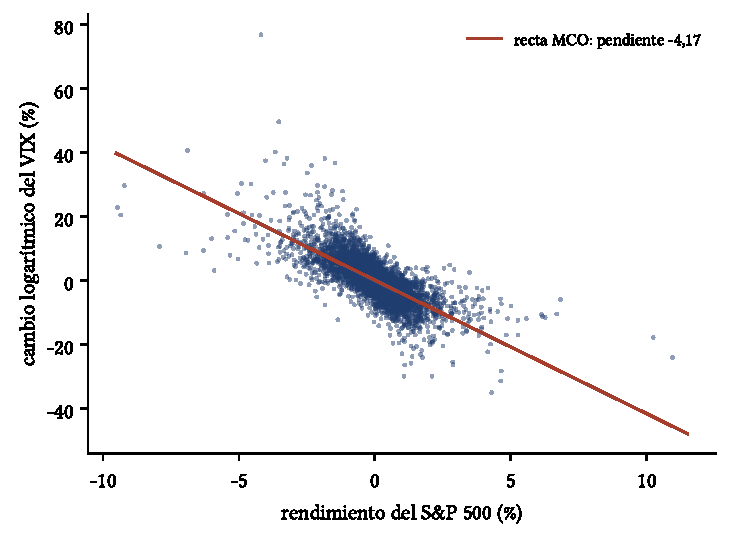
\includegraphics[width=0.62\linewidth]{graficos/cap10_ej01_dispersion.pdf}
\caption{Rendimiento diario del S\&P 500 frente al cambio logarítmico del VIX del mismo día (1999--2018).}
\label{fig:varvixdisp}
\end{figure}

\begin{conclusion}
El VAR(2) es estable. Casi toda la interacción entre el S\&P 500 y el VIX ocurre dentro del mismo día; la
dinámica rezagada es débil. Eso anticipa que el orden de Cholesky será decisivo para las respuestas al impulso.
\end{conclusion}
\end{ejresuelto}

\begin{ejresuelto}{Causalidad de Granger en dos pares de mercados}\label{ej:granger}
\enunciado Contraste la causalidad de Granger en ambas direcciones: (a) entre $r_t$ y $\Delta v_t$ con VAR(2) y
VAR(7); (b) entre las carteras mensuales S1V3 (pequeña) y S5V3 (grande) de French, con el orden elegido por BIC
y por AIC. Use la prueba $F$ y la de Wald robusta.

\solucion
\paso{Paso 1. S\&P 500 y VIX.}
\begin{center}\small
\begin{tabular}{@{}llrrrr@{}}
\toprule
Hipótesis nula & $p$ & $F$ & valor $p$ & Wald HC0 & valor $p$ \\
\midrule
$\Delta v$ no causa a $r$ & 2 & 1,870 & 0,154 & 1,947 & 0,378 \\
$r$ no causa a $\Delta v$ & 2 & 2,666 & 0,070 & 3,899 & 0,142 \\
$\Delta v$ no causa a $r$ & 7 & 1,496 & 0,164 & 6,296 & 0,506 \\
$r$ no causa a $\Delta v$ & 7 & 1,571 & 0,139 & 8,243 & 0,312 \\
\bottomrule
\end{tabular}
\end{center}
Ninguna hipótesis se rechaza al 5\,\%. El rendimiento de ayer ayuda marginalmente a predecir el cambio del VIX
con la prueba $F$ ($p=0{,}070$), pero la evidencia desaparece con la prueba robusta ($p=0{,}142$): la prueba
clásica sobrestima la significancia porque los residuos son muy heterocedásticos.

\paso{Paso 2. Carteras pequeña y grande.} El BIC elige $p=1$ y el AIC $p=5$.
\begin{center}\small
\begin{tabular}{@{}llrrrr@{}}
\toprule
Hipótesis nula & $p$ & $F$ & valor $p$ & Wald HC0 & valor $p$ \\
\midrule
grande no causa a pequeña & 1 & 3,702 & 0,055 & 2,472 & 0,116 \\
pequeña no causa a grande & 1 & 0,333 & 0,564 & 0,276 & 0,600 \\
grande no causa a pequeña & 5 & 2,083 & 0,066 & 5,615 & 0,346 \\
pequeña no causa a grande & 5 & 0,863 & 0,505 & 4,356 & 0,499 \\
\bottomrule
\end{tabular}
\end{center}
La asimetría que encontramos en el Capítulo~\ref{cap:eficiencia} reaparece (el valor $p$ en el sentido
grande$\to$pequeña es mucho menor que en el sentido contrario), pero no alcanza el 5\,\% y se debilita con la
prueba robusta. Para $p=1$, la prueba $F$ con una restricción es el cuadrado del estadístico $t$ de la
regresión del Ejercicio~\ref{ej:adelanto}: $1{,}924^2=3{,}702$.

\codigoweb{cap10_ej02}
\salidaR{cap10_ej02_R.txt}
\lectura{cap10_ej02}

\RvsPy Nuestra prueba $F$ usa una sola ecuación, con $n-q=815$ grados de libertad en el denominador.
\texttt{test\_causality} de \texttt{statsmodels} usa el sistema completo y $K(n-q)=1\,630$ grados de libertad;
el estadístico es el mismo ($3{,}702$) y el valor $p$ cambia en la cuarta decimal ($0{,}0545$ frente a
$0{,}0547$). La prueba robusta no está en \texttt{statsmodels} para el VAR, así que la programamos con la matriz
de White en los dos lenguajes.

\begin{conclusion}
En estos datos no hay causalidad de Granger significativa. Es lo esperable en mercados líquidos: si el pasado de
un precio predijera claramente a otro, los inversionistas lo aprovecharían. Además, la heterocedasticidad
puede hacer parecer significativas relaciones que no lo son, por lo que conviene reportar siempre la versión
robusta.
\end{conclusion}
\end{ejresuelto}

\begin{ejresuelto}{Respuestas al impulso entre el S\&P 500 y el VIX}\label{ej:irfvix}
\enunciado Con el VAR(2) del Ejercicio~\ref{ej:varvix}, calcule las respuestas ortogonalizadas con el orden
$(r,\Delta v)$ y con el orden $(\Delta v,r)$, y bandas \emph{bootstrap} al 90\,\% con 500 réplicas para el
primero. Calcule la respuesta acumulada del VIX a un choque positivo en el S\&P 500.

\solucion
\paso{Paso 1. Factor de Cholesky.} Con el orden $(r,\Delta v)$:
\begin{align*}
  p_{11} &= \sqrt{1{,}4376}=1{,}1990,\\
  p_{21} &= \frac{-5{,}9884}{1{,}1990}=-4{,}9945,\\
  p_{22} &= \sqrt{46{,}0708-(-4{,}9945)^2}\\
         &= \sqrt{46{,}0708-24{,}9450}\\
         &= \sqrt{21{,}1258}=4{,}5963 .
\end{align*}
Un choque de una desviación estándar en el S\&P 500 ($+1{,}20$\,\%) baja el VIX $4{,}99$\,\% el mismo día.

\paso{Paso 2. Dinámica.}
\begin{center}\small
\begin{tabular}{@{}rrrrr@{}}
\toprule
$h$ & $r\leftarrow r$ & $\Delta v\leftarrow r$ & $r\leftarrow\Delta v$ & $\Delta v\leftarrow\Delta v$ \\
\midrule
0  & 1,1990 & $-4{,}9945$ & 0,0000 & 4,5963 \\
1  & $-0{,}0895$ & 0,5328 & $-0{,}0253$ & $-0{,}2856$ \\
2  & $-0{,}0558$ & 0,3894 & $-0{,}0185$ & $-0{,}1581$ \\
5  & $-0{,}0002$ & 0,0058 & $-0{,}0006$ & 0,0009 \\
\bottomrule
\end{tabular}
\end{center}
Tras la caída inicial, el VIX rebota: sube $0{,}53$\,\% el día siguiente y $0{,}39$\,\% el segundo, y las bandas
excluyen el cero (por ejemplo, $[0{,}367;\ 0{,}696]$ en $h=1$ en R). La respuesta acumulada a 10 días es
$-4{,}16$\,\%: el VIX devuelve en dos días una sexta parte de su caída. La respuesta del S\&P 500 a un choque en
el VIX es pequeña y su banda incluye el cero o lo roza.

\paso{Paso 3. El orden importa.} Con el orden $(\Delta v,r)$, la correlación contemporánea se atribuye al VIX:
un choque en el VIX baja el S\&P 500 $0{,}88$\,\% en el impacto, y el choque ``propio'' del S\&P 500 ya no mueve
al VIX en ese período. Las respuestas en $h\ge1$ también cambian (Figura~\ref{fig:irfvix}). Con una correlación de
$-0{,}74$ entre innovaciones, el orden decide casi toda la historia: los datos no distinguen si es el mercado el
que mueve al VIX o al revés.

\codigoweb{cap10_ej03}
\salidaR{cap10_ej03_R.txt}
\lectura{cap10_ej03}

\RvsPy En R, \texttt{chol()} devuelve la triangular \emph{superior} $R$ con $R'R=\Sigma$, por lo que usamos
$P=R'$; \texttt{np.linalg.cholesky} devuelve directamente la inferior. Las respuestas puntuales coinciden con
\texttt{orth\_ma\_rep} de \texttt{statsmodels}. Las bandas \emph{bootstrap} difieren entre lenguajes en la
segunda o tercera cifra porque los generadores de números aleatorios no son los mismos, aunque usen la misma
semilla. Por ejemplo, la banda de $r\leftarrow\Delta v$ en $h=1$ es $[-0{,}0538;\ 0{,}0023]$ en R y
$[-0{,}0513;\ -0{,}0005]$ en Python: un resultado que está en el límite de la significancia puede cambiar de lado
según la simulación, lo que es en sí mismo una advertencia.

\begin{figure}[ht]
\centering
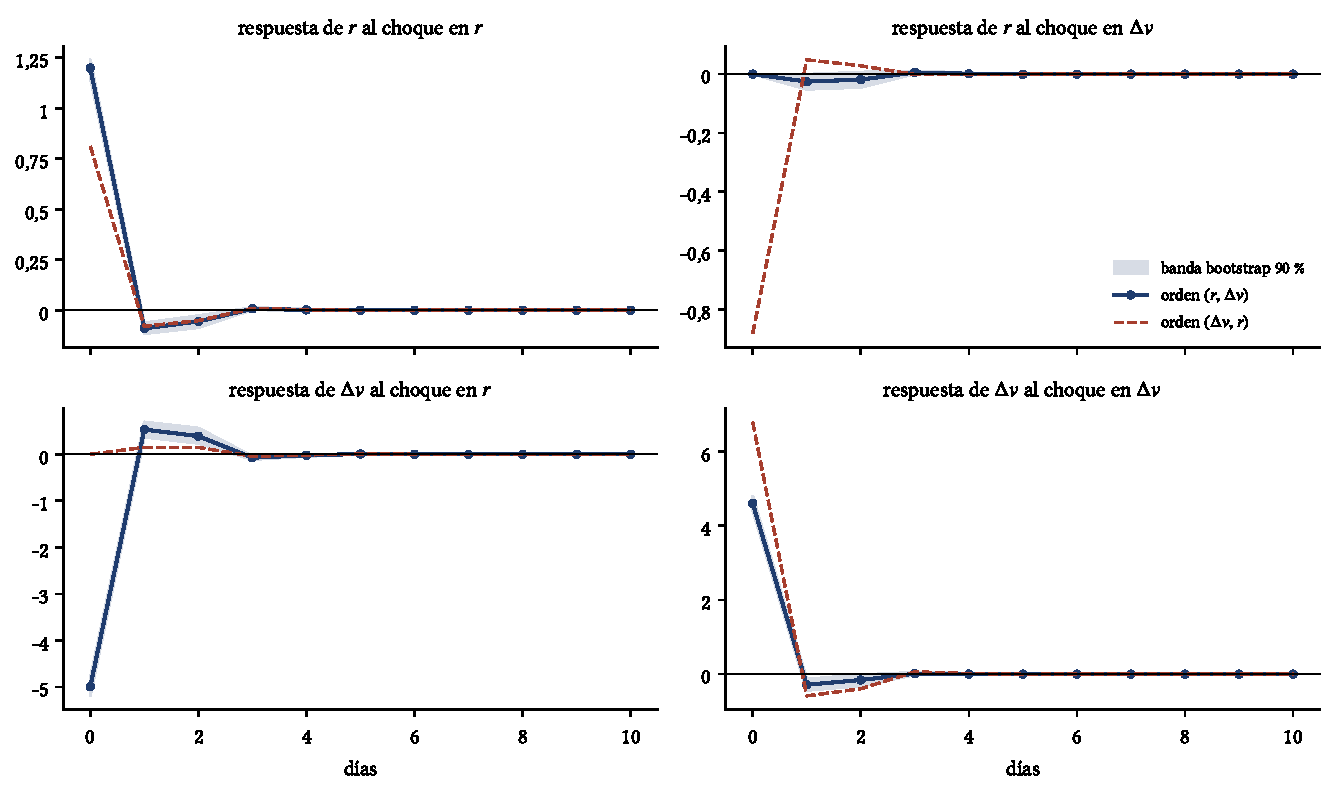
\includegraphics[width=\linewidth]{graficos/cap10_ej03_irf.pdf}
\caption{Respuestas ortogonalizadas del VAR(2) para el S\&P 500 ($r$) y el VIX ($\Delta v$), con la banda
\emph{bootstrap} al 90\,\% para el orden $(r,\Delta v)$ y la respuesta puntual con el orden inverso.}
\label{fig:irfvix}
\end{figure}

\begin{conclusion}
Un choque positivo al S\&P 500 reduce el VIX de inmediato, y el VIX corrige parcialmente en los dos días
siguientes. Como la relación es casi toda contemporánea, las respuestas dependen de forma crítica del orden de
Cholesky; conviene reportar ambos órdenes cuando la teoría no da uno.
\end{conclusion}
\end{ejresuelto}

\begin{ejresuelto}{Inflación, tasas de interés y acciones en EE.\,UU.}\label{ej:varmacro}
\enunciado Con datos mensuales de EE.\,UU.\ (1960--2023) estime un VAR con la inflación ($\mathit{inf}$, cambio
logarítmico del IPC en porcentaje), el cambio en la tasa de los bonos a 10 años ($\mathit{dtasa}$, en puntos
porcentuales) y el rendimiento total del S\&P 500 ($\mathit{ret}$, en porcentaje). Elija el orden, contraste la
causalidad de Granger y calcule respuestas y descomposición de la varianza con el orden
$(\mathit{inf},\mathit{dtasa},\mathit{ret})$.

\solucion
\paso{Paso 1. Orden.} Con $T=761$ meses y $p_{\max}=12$, el AIC elige 12, el BIC 1 y el HQ 2. Usamos $p=2$,
un compromiso que conserva algo de dinámica sin sobreajustar. El orden de Cholesky refleja que el IPC y las tasas
de largo plazo se mueven más despacio que las acciones: suponemos que las acciones pueden reaccionar en el mes
a la inflación y a las tasas, pero no al revés.

\paso{Paso 2. Causalidad de Granger.}
\begin{center}\small
\begin{tabular}{@{}lrrrr@{}}
\toprule
Hipótesis nula & $F$ & valor $p$ & Wald HC0 & valor $p$ \\
\midrule
$\mathit{dtasa}$ no causa a $\mathit{inf}$ & 5,144 & 0,006 & 9,103 & 0,011 \\
$\mathit{ret}$ no causa a $\mathit{inf}$ & 4,991 & 0,007 & 4,447 & 0,108 \\
$\mathit{inf}$ no causa a $\mathit{dtasa}$ & 8,435 & 0,000 & 12,062 & 0,002 \\
$\mathit{ret}$ no causa a $\mathit{dtasa}$ & 9,799 & 0,000 & 14,474 & 0,001 \\
$\mathit{inf}$ no causa a $\mathit{ret}$ & 1,347 & 0,261 & 2,704 & 0,259 \\
$\mathit{dtasa}$ no causa a $\mathit{ret}$ & 7,239 & 0,001 & 12,979 & 0,002 \\
$\mathit{inf}$ y $\mathit{dtasa}$ no causan a $\mathit{ret}$ & 4,866 & 0,001 & 15,663 & 0,004 \\
\bottomrule
\end{tabular}
\end{center}
A diferencia de los datos diarios, aquí sí hay causalidad de Granger robusta: los cambios pasados en la tasa de
interés ayudan a predecir el rendimiento de las acciones, y la inflación y las tasas se predicen mutuamente.

\paso{Paso 3. Respuestas del rendimiento.} Un choque de una desviación estándar en la tasa
($0{,}25$ puntos) reduce el rendimiento del S\&P 500 en $0{,}24$ puntos en el mes y en $0{,}52$ el mes
siguiente; uno en la inflación lo reduce $0{,}27$ puntos al mes siguiente. A 24 meses, las respuestas acumuladas
son $-0{,}85$ y $-0{,}56$ puntos (Figura~\ref{fig:varmacro}). Que la reacción sea mayor un mes después que en el
mes del choque se explica en parte porque el IPC se publica con rezago y porque los precios de la base de
Shiller son promedios mensuales.

\paso{Paso 4. Descomposición de la varianza.} En $h=1$ se usa la fila de $\mathit{ret}$ en $\Theta_0$:
\begin{align*}
  (\theta_{31,0},\ \theta_{32,0},\ \theta_{33,0}) &= (-0{,}0228;\ -0{,}2356;\ 3{,}4648),\\[4pt]
  \mathrm{ECM}_{\mathit{ret}}(1) &= 0{,}0228^2+0{,}2356^2+3{,}4648^2\\
                                &= 0{,}0005+0{,}0555+12{,}0048\\
                                &= 12{,}0609,\\[4pt]
  \omega_{\mathit{ret},\mathit{dtasa}}(1) &= \frac{0{,}0555}{12{,}0609}=0{,}0046 .
\end{align*}
Es decir, el choque de tasa explica el 0,46\,\% de la varianza del error a un mes.
A 24 meses, la inflación explica el $0{,}78$\,\% y la tasa el $2{,}78$\,\% de la varianza del error de pronóstico
del rendimiento; el $96{,}44$\,\% restante viene de sus propios choques.

\codigoweb{cap10_ej04}
\salidaR{cap10_ej04_R.txt}
\lectura{cap10_ej04}

\RvsPy La descomposición de \texttt{statsmodels} (\texttt{fevd}) coincide con la nuestra. Atención con los
índices: nuestra función guarda los horizontes $h=0,1,\dots$, de modo que la proporción a $h$ períodos está en la
posición $h-1$ en Python y en la fila $h$ en R.

\begin{figure}[ht]
\centering
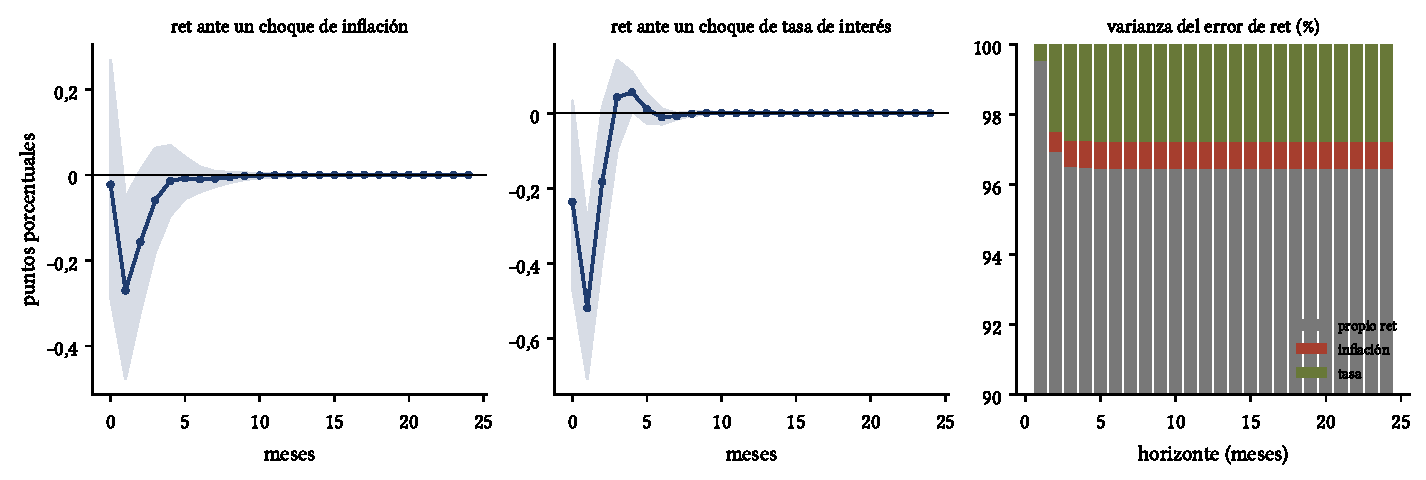
\includegraphics[width=\linewidth]{graficos/cap10_ej04_macro.pdf}
\caption{Respuesta del rendimiento del S\&P 500 a choques de inflación y de tasa de interés (con banda
\emph{bootstrap} al 90\,\%) y descomposición de la varianza de su error de pronóstico; el eje vertical del panel
derecho empieza en 90\,\%.}
\label{fig:varmacro}
\end{figure}

\begin{conclusion}
Las tasas de interés y la inflación predicen las acciones de forma estadísticamente robusta, con el signo que
predice la teoría (más inflación y más tasa, menor rendimiento). Pero la magnitud es pequeña: explican menos del
4\,\% de la incertidumbre sobre el rendimiento del mes siguiente.
\end{conclusion}
\end{ejresuelto}

\begin{ejresuelto}{¿Pronostica el VAR mejor que la media histórica?}\label{ej:varfuera}
\enunciado Para el rendimiento mensual de la cartera pequeña S1V3, genere pronósticos a un mes desde enero de
1983 con ventana creciente usando: (i) la media histórica, (ii) un AR(1) y (iii) la ecuación de la cartera
pequeña de un VAR(1) con la grande. Calcule el $R^2$ fuera de muestra y aplique la prueba de Clark y West.

\solucion
\paso{Paso 1. El $R^2$ fuera de muestra.} Campbell y Thompson (2008) lo definen respecto de la media histórica:
\[
  R^2_{\text{FM}}=1-\frac{\sum_t(y_t-\hat y_t^{\text{modelo}})^2}{\sum_t(y_t-\bar y_t)^2},
\]
donde $\bar y_t$ es la media con datos hasta $t-1$. Es positivo si el modelo pronostica mejor que la media. Con
411 meses de evaluación (enero de 1983 a marzo de 2017), los errores cuadráticos medios son 30,72 (media), 30,09
(AR) y 30,00 (VAR):
\begin{align*}
  R^2_{\text{FM}}(\text{AR}) &= 1-\frac{30{,}0903}{30{,}7166}=0{,}0204,\\
  R^2_{\text{FM}}(\text{VAR}) &= 1-\frac{29{,}9954}{30{,}7166}=0{,}0235,
\end{align*}
es decir, 2,04\,\% y 2,35\,\%.

\paso{Paso 2. Prueba de Clark y West.} Cuando un modelo está anidado en otro, la prueba de Diebold-Mariano está
sesgada contra el modelo grande, que debe estimar parámetros que bajo la nula valen cero. Clark y West (2007)
corrigen ese sesgo con
\[
  f_t=e_{1t}^2-\bigl[e_{2t}^2-(\hat y_{1t}-\hat y_{2t})^2\bigr],
\]
y contrastan unilateralmente que $\E[f_t]=0$ con un estadístico $t$ de Newey-West. Resultados: media frente a
AR(1), $t=2{,}73$ ($p=0{,}003$); media frente a VAR(1), $t=2{,}79$ ($p=0{,}003$); AR(1) frente a VAR(1), $t=1{,}17$
($p=0{,}121$). Los rendimientos pasados de la cartera pequeña ayudan a pronosticarla fuera de muestra; agregar la
cartera grande no mejora significativamente.

\paso{Paso 3. Estabilidad en el tiempo.} El $R^2_{\text{FM}}$ es de $5{,}69$\,\% (AR) y $5{,}09$\,\% (VAR) en
1983--1999, pero de $-0{,}58$\,\% y $0{,}38$\,\% en 2000--2017. La Figura~\ref{fig:varfuera} muestra que la ventaja se
acumula hasta 2000 y luego se estanca: la predictibilidad de las acciones pequeñas casi desapareció en las
últimas dos décadas.

\codigoweb{cap10_ej05}
\salidaR{cap10_ej05_R.txt}
\lectura{cap10_ej05}

\RvsPy El bucle de ventana creciente es idéntico: en R reestimamos con \texttt{lm} y en Python con
\texttt{np.linalg.lstsq}. Cuidado con los índices: en R el primer mes pronosticado es la fila
\texttt{which(f\$dates == "1983-01")}; en Python, que cuenta desde cero, \texttt{np.flatnonzero(...)[0]}, y en
ambos casos la estimación usa solo datos anteriores.

\begin{figure}[ht]
\centering
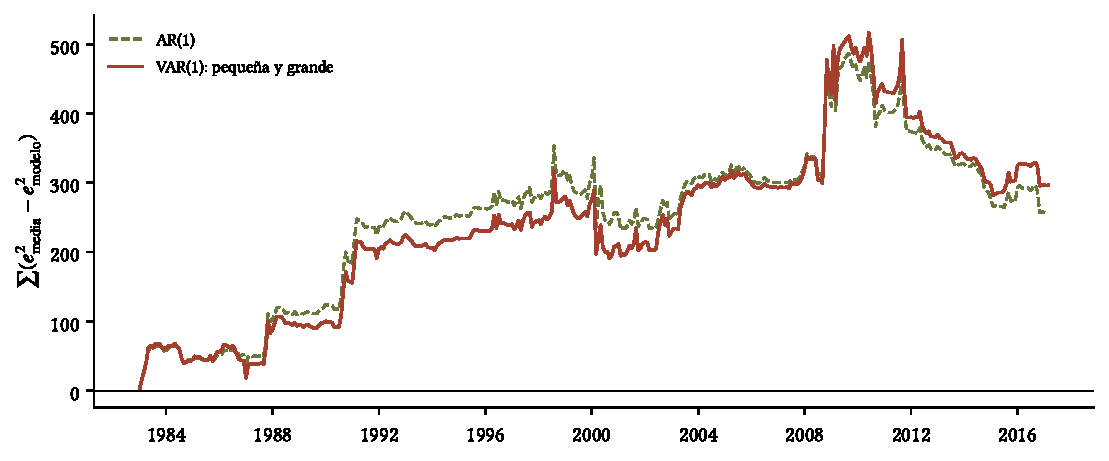
\includegraphics[width=0.88\linewidth]{graficos/cap10_ej05_fuera_muestra.pdf}
\caption{Diferencia acumulada entre los errores cuadráticos de la media histórica y los del modelo. Una curva
que sube indica que el modelo pronostica mejor; después de 2000 la curva deja de subir.}
\label{fig:varfuera}
\end{figure}

\begin{conclusion}
Un modelo dinámico sencillo pronostica la cartera pequeña algo mejor que la media histórica, con significancia
estadística. Pero la ganancia se concentra antes de 2000, y la información de la cartera grande no aporta casi
nada adicional. En pronóstico financiero, los modelos parsimoniosos suelen ser tan buenos como los complejos.
\end{conclusion}
\end{ejresuelto}

% ---------------------------------------------------------------------
\section{Ejercicios propuestos}
% ---------------------------------------------------------------------

\begin{enumerate}[label=\textbf{\thechapter.\arabic*},leftmargin=*,itemsep=6pt]
  \item Escriba la matriz compañera de un VAR(2) bivariado y demuestre que, si $A_2=0$, sus autovalores son los
  de $A_1$ más dos ceros.

  \item Para el VAR(1) con $A_1=\bigl[\begin{smallmatrix}0{,}5&0{,}1\\0{,}3&0{,}6\end{smallmatrix}\bigr]$, calcule
  los autovalores y $\Psi_2$. \textit{Respuesta: $0{,}7303$ y $0{,}3697$;
  $\Psi_2=\bigl[\begin{smallmatrix}0{,}28&0{,}11\\0{,}33&0{,}39\end{smallmatrix}\bigr]$.}

  \item Con $\Sigma=\bigl[\begin{smallmatrix}4&1\\1&2\end{smallmatrix}\bigr]$, calcule el factor de Cholesky
  con el orden $(y_1,y_2)$ y con el orden $(y_2,y_1)$. \textit{Respuesta:
  $\bigl[\begin{smallmatrix}2&0\\0{,}5&1{,}3229\end{smallmatrix}\bigr]$; con el orden inverso, $y_2$ recibe
  $\sqrt2=1{,}4142$ en su propio choque e $y_1$ recibe $0{,}7071$ y $1{,}8708$.}

  \item Demuestre que, en un VAR bivariado, si $y_2$ no causa a $y_1$ en el sentido de Granger, entonces
  $\Psi_i[1,2]=0$ para todo $i$.

  \item Demuestre que la descomposición de la varianza a un período con el orden $(y_1,y_2)$ atribuye el
  100\,\% de la varianza de $y_1$ a su propio choque.

  \item \emph{(Simulación.)} Simule 1\,000 muestras de $T=200$ observaciones de dos paseos aleatorios
  independientes y estime un VAR(1) en niveles. ¿Con qué frecuencia rechaza la prueba $F$ al 5\,\% la hipótesis
  de no causalidad? Compare con un VAR en primeras diferencias.

  \item \emph{(Con datos del BCRP.)} Estime un VAR mensual con la inflación, el tipo de cambio sol/dólar y la
  tasa de referencia del BCRP. Elija un orden de Cholesky justificado y calcule la respuesta de la inflación a
  un choque cambiario (traspaso del tipo de cambio).

  \item \emph{(Con datos.)} Repita el Ejercicio~\ref{ej:irfvix} con un VAR de tres variables que agregue el
  rendimiento diario del Brent. ¿Qué fracción de la varianza del error de pronóstico del S\&P 500 explican los
  choques del petróleo?
\end{enumerate}

% ---------------------------------------------------------------------
\section{Resumen de fórmulas}
% ---------------------------------------------------------------------

\begin{table}[H]
\centering\small
\begin{tabular}{@{}ll@{}}
\toprule
Concepto & Fórmula \\
\midrule
VAR($p$) & $\mathbf y_t=\mathbf c+\sum_{j=1}^{p}A_j\mathbf y_{t-j}+\mathbf u_t$,\quad $\E[\mathbf u_t\mathbf u_t']=\Sigma$ \\
Estabilidad & autovalores de la matriz compañera $F$ con $|\lambda|<1$ \\
Medias móviles & $\Psi_0=I$,\quad $\Psi_i=\sum_{j=1}^{\min(i,p)}A_j\Psi_{i-j}$ \\
Estimador & $\hat B=(X'X)^{-1}X'Y$ (MCO por ecuación $=$ MCG) \\
Criterios & $\ln|\tilde\Sigma_p|+c_n\,(pK^2+K)/n$;\quad $c_n=2,\ \ln n,\ 2\ln\ln n$ \\
Granger & $F=[(\mathrm{SRC}_r-\mathrm{SRC}_u)/r]/[\mathrm{SRC}_u/(n-q)]$ \\
Cholesky & $PP'=\Sigma$,\quad $\Theta_i=\Psi_iP$ \\
Descomposición & $\omega_{kj}(h)=\sum_{i<h}\theta_{kj,i}^2\big/\sum_{i<h}\sum_m\theta_{km,i}^2$ \\
$R^2$ fuera de muestra & $1-\sum(y_t-\hat y_t)^2/\sum(y_t-\bar y_t)^2$ \\
\bottomrule
\end{tabular}
\caption{Fórmulas principales del Capítulo 10.}
\end{table}

\section*{Referencias}
\begin{itemize}[leftmargin=*]
  \item Campbell, J. Y. y Thompson, S. B. (2008). Predicting excess stock returns out of sample: Can anything beat
        the historical average? \emph{Review of Financial Studies}, 21(4), 1509--1531.
  \item Clark, T. E. y West, K. D. (2007). Approximately normal tests for equal predictive accuracy in nested
        models. \emph{Journal of Econometrics}, 138(1), 291--311.
  \item Granger, C. W. J. (1969). Investigating causal relations by econometric models and cross-spectral
        methods. \emph{Econometrica}, 37(3), 424--438.
  \item Kilian, L. y Lütkepohl, H. (2017). \emph{Structural Vector Autoregressive Analysis}. Cambridge University
        Press.
  \item Lütkepohl, H. (2005). \emph{New Introduction to Multiple Time Series Analysis}. Springer.
  \item Pesaran, H. H. y Shin, Y. (1998). Generalized impulse response analysis in linear multivariate models.
        \emph{Economics Letters}, 58(1), 17--29.
  \item Sims, C. A. (1980). Macroeconomics and reality. \emph{Econometrica}, 48(1), 1--48.
\end{itemize}
